\documentclass[11pt,a4paper]{article}
\usepackage[utf8]{inputenc}
\usepackage[margin=2.5cm]{geometry}

\usepackage{microtype}
\usepackage{mathpazo} % nice fonts
\usepackage{xcolor}
\usepackage[unicode=true,pdftex,pdfa,colorlinks=true]{hyperref}

\usepackage{amsmath}
\usepackage{makecell}
\usepackage{multirow}

\usepackage{graphicx}

\usepackage{tikz}
\usetikzlibrary{automata,positioning}
\usepackage{pgf}
\usepackage{pgfplots}
\pgfplotsset{compat=1.15}

\usepackage{listings}
\usepackage{color}

\newtheorem{definition}{Definition}
\newtheorem{proof}{Proof}
\newtheorem{theorem}{Theorem}

\begin{document}

\hypersetup{
  pdftitle={Design specification of the PRIViLEDGE update mechanism},
  breaklinks=true,
  linkcolor={blue},
  citecolor={blue},
  urlcolor={blue},
  linkbordercolor={white},
  citebordercolor={white},
  urlbordercolor={white}
}

\title{
  Decentralized software updates for stake-based ledgers\\
  \large Design specification
  of the PRIViLEDGE update mechanism\\
}

\author{
  Nikos Karagiannidis\\
  {\small \texttt{nikos.Karagiannidis@iohk.io}}\\
  \and
  Damian Nadales \\
  {\small \texttt{damian.nadales@iohk.io}}\\
}

\date{\today}

\maketitle

\section*{List of Contributors}
\label{acknowledgements}

Michele Ciampi, Dionysis Zindros, Aggelos Kiayias.

\tableofcontents
\listoffigures
\listoftables

\section{Purpose}
\label{sec:purpose}

% What is the purpose of this document?
This document presents the design of a decentralized governance mechanism for
updating public blockchain systems.
% What is governance.
In this context, updating refers to the set of changes by which the blockchain
evolves. Governance deals with the set of rules by which the decisions that
pertain to this update
process are made.
% When is governance decentralized?
We say that blockchain governance is decentralized when the community can
leverage on these rules to determine the direction in which said blockchain
evolves. A decentralized blockchain with a
centralized governance scheme is an oxymoron.
% Why people should care about the problems stated in this document?
Thus a decentralized update mechanism is crucial for achieving a decentralized
blockchain.

% Why people should care about this document? What is the target audience?
This document is intended for stakeholders interested realizing an
implementation of a decentralized governance mechanism for blockchains.

% What does this document contains
This document features a breakdown of the requirements for achieving
decentralization of the update mechanism in a blockchain, and describes a design
that satisfies these requirements.

% Who funded this work?
The work presented here was funded by the PRIViLEDGE project~\cite{priviledge}.

% Mention Voltaire, and how this document relates to it.
The Voltaire era of Cardano will provide a governance system for the Cardano
network to become a self-sustaining system, no longer under IOHK's management.
The work presented here can be used as the base for the governance system of the
Voltaire era.

\section{Requirements}
\label{sec:requirements}

This section presents the requirements of an update mechanism for achieving
decentralized governance of a blockchain.

\subsection{Open}
\label{sec:open-participation}

In the absence of malicious actors, we would wish that anybody who can
participate the blockchain protocol by submitting transactions can participate
in the update process. However allowing this would open the door for spam
attacks: if the barrier for submitting update proposals is as low as submitting
regular transactions, then we risk having a large number of bogus update
proposals being submitted that will overwhelm the human actors that have to
review these proposals.

In light of the risk presented in the preceding paragraph, we require that the
group of people that can participate in the update process should be as broad as
possible, but not broader. This means that:
\begin{itemize}
\item Restrictions on the group of people that can submit update proposals
  should be as loose as possible.
\item Any participant that can submit a common transaction should be able to
  vote on update proposals.
\end{itemize}

\subsection{Democratic}
\label{sec:decentr-decis-making}

All major decisions in the life cycle of a system update should be made by the
community, via a secure voting mechanism.

\subsection{Protocol driven}
\label{sec:protocol-driven}

The update protocol should be an on-chain process, which is automatically
enforced by the ledger rules of the blockchain.

\subsection{Transparent and auditable}
\label{sec:transp-audit}

Anybody should be able to answer \emph{when}, \emph{why}, and \emph{how} the
system has evolved the way it has. The systems' update history should be:
\begin{itemize}
\item open to everyone, and
\item stored in a tamper-free global ledger.
\end{itemize}

\subsection{Secure}
\label{sec:secure}
Security for decentralized blockchain updates pertains to two main areas: a)
the
decentralized decision making process and b) the activation of the changes on
the blockchain. Therefore, one has to define security in this context and then
propose a mechanism that ensures the said security.

\subsection{Performant and scalable}
\label{sec:performant-scalable}

The impact of the update protocol should have minimal impact on the:
\begin{itemize}
\item transaction throughput,
\item blockchain size, and
\item block processing time.
\end{itemize}

\subsection{Metadata-driven}
\label{sec:metadata-driven}

Not all updates are the same. For instance some updates might be more urgent
than others, some updates might depend on a specific protocol version, some
updates might take longer than others, for some updates a higher approval
threshold is more appropriate etc. Therefore, it should be possible to
specify proposal-dependent features that the protocol must enforce.

\subsection{Consistent}
\label{sec:cons-update-logic}

The update protocol should define and automatically enforce a policy that is
consistent with the metadata of the update proposals and ensure that the
applied updates always leave the system in a consistent state. So for instance,
the update protocol should obey the priorities of proposals and their version
dependencies.

\section{Design}
\label{sec:design}

\subsection{Update types}
\label{sec:update-types}

% What is an update? How are updates related to the blockchain evolution and/or
% how are they related to governance.
Updates are the means by which the blockchain system and related ecosystem (e.g.
wallets, explorers) can evolve. We distinguish the following update types:
\begin{description}
\item[Protocol] These updates affect the consensus rules by which nodes agree on
  a common blockchain. Protocol updates fall in one of the following two
  categories:
  \begin{description}
  \item[Signaled] An update is said to be \emph{signaled} if the nodes must
    signal they readiness to run the new protocol. For instance, when a new
    protocol requires the nodes to download and install new software, the
    protocol must have a way to determine when a sufficient majority of them
    have upgraded to the new version.
  \item[Non-signaled] An update is said to be \emph{non-signaled} if the nodes
    can move to the new protocol version without needing to know if other nodes
    are ready to move to said version as well.
    %
    In this kind of updates we assume the nodes are already running a version of
    the software that can automatically switch to the new protocol. This switch,
    called activation takes place at a time point set by the update mechanism
    (e.g., the next epoch after the approval of the update).
    %
    An example of non-signaled protocol updates is a \emph{parameters-update}.
    In a parameters-update, the nodes have already the logic for handling the
    parameters, and only the values of these parameters change after an update
    is activated.
  \end{description}
\item[Non-protocol] These updates do not affect the consensus rules. The current
  design does not restrict the nature of these updates. It is up to the ledger
  layer to react to these updates accordingly. They might include:
  \begin{itemize}
  \item Updates to the software that runs on the blockchain nodes, which does
    not affect the protocol. Examples of such updates might include performance
    or usability improvements.
  \item Funds transfers. For instance an update proposal might involve funding
    the development of a certain feature.
  \item Updates to other components of the blockchain ecosystem.
  \end{itemize}
\item[Cancellation] These are special kind of update proposals that can be used
  to cancel other \emph{approved} protocol update proposals\footnote{For
    non-approved proposals the expert pools can simply reject said update}.
\end{description}

Note that, according to the preceding definition, an update that requires the
node to download and install new software to run a \emph{new protocol}, and that
\emph{also} updates protocol parameters is considered a signaled protocol
update.

\subsection{The lifecycle of a decentralized update}
\label{sec:phases-an-update}

The update protocol described in this document aims at capturing the whole life
cycle of an update.
%
We distinguish the following \emph{phases} in the life cycle of an update:

\begin{description}
\item[Ideation] In this phase, the idea for an update is presented to the
  stakeholders in the form of an \emph{system improvement proposal} (SIP). An
  SIP is voted by the system's stakeholders. An SIP is materialized in the form
  of a (well-structured) text document, and as such, once it is approved it
  does not have any effect
  in the system until its implementation gets activated.
\item[Implementation] In case an update requires an implementation, this is the
  phase where it takes place. Some updates like parameter updates, or fund
  transfers do not require an implementation. This phase is not captured by the
  protocol proposed in this document, and we assume it takes place entirely
  off-chain.
\item[Approval] In this phase, the information about the implementation of an
  SIP is submitted to the chain. Henceforth, the implementation update proposal
  is referred to as UP (\emph{update proposal}). As in the ideation phase, the
  stakeholders vote on the
  implementation.
\item[Activation] Once an protocol update implementation is approved, it moves
  to the activation phase, where it might become the current protocol version,
  according to the rules described in Section~\ref{sec:activation}. Non-protocol
  updates are not activated. Their approval is registered by the protocol and
  it is up to the ledger layer to act on them.
\end{description}

In Sections~\ref{sec:ideation} and \ref{sec:approval} we describe the
information that update proposals must submit to the blockchain. Stakeholders
vote on SIPs and their implementations, and thus we describe the voting
mechanism in Section~\ref{sec:voting}. Stakeholders can delegate their vote. The
delegation mechanism and the problems it addresses are described in
Section~\ref{sec:delegation}.

Once an implementation is approved, if it refers to protocol changes it has to
be \emph{activated}. In Section~\ref{sec:activation} we describe the activation
protocol.

When designing a decentralized update protocol for PoS blockchain systems, we
must determine a stake \emph{threshold} to reach on verdict on whether a
proposal should be approved or rejected. This problem is described and addressed
in Section~\ref{sec:threshold-analysis}.

Finally, the update protocol should not have a large impact on the normal
operation of the blockchain it runs on. In
Section~\ref{sec:performance-analysis} we turn our attention to the performance
analysis of the protocol described in this document.

\subsection{Delegation}
\label{sec:delegation}

% When we describe how votes are counted we need to talk about delegation. Hence
% we must first talk about what delegation is.
In the proof-of-stake blockchain system we assume in the current design, each
stakeholder has the right to participate in the update protocol.
%
In this section, we discuss the delegation of the voting rights. As we will see
next, this delegation serves various purposes and copes with several practical
challenges.

%%
%% Delegation protocol
%%
\subsubsection{Delegation for technical expertise}
\label{sec:deleg-techn-expert}

One of the first practical challenges in decentralized governance of blockchains
is the requirement of having participants with the sufficient \emph{technical
  expertise} to assess a specific software update proposal.
%
Even at the SIP level, many of the software update proposals are too technical
for the majority of stake to understand.
%
Moreover, during the UP approval phase, the approver is called for approving or
rejecting the submitted source code, which is certainly a task only for experts.

Our proposed solution to this problem is to enable delegation to participants
that posses the required technical expertise.
%
Stakeholders will be able to delegate their right to participate in the update
protocol to an \emph{expert pool}. The proposed delegation to an expert pool
comprises the following distinct responsibilities:
\begin{itemize}
\item Voting for a specific SIP.
\item Voting for a given category of SIPs.
\item Voting for any SIP.
\item Approving a specific UP.
\item Approving a given category of UPs.
\item Approving any UP.
\end{itemize}
We distinguish delegation for voting for a SIP document and for approving an UP.
We could have defined delegation for SIP voting to imply also the approval of
the corresponding UP. However, since both have a totally different scope, there
might be a need to delegate to different expert pools to vote on them. An SIP is
a document that, among other things, justifies an update proposal, and the
expert who is called to vote for or against a specific SIP must know the
road-map of the system very well. On the other hand, the approval of a UP is a very
technical task, which requires reviewing and testing of code
against some requirements (i.e.,the corresponding SIP) and has nothing
to do with the software road-map.

\subsubsection{Delegation for specialization}
\label{sec:deleg-spec}

There are special categories of software updates, like security fixes.
%
Common sense dictates that security fixes are software updates which:
\begin{enumerate}
\item have a high priority, and
\item require significant technical expertise to be evaluated.
\end{enumerate}
Therefore, having a special expert pool as a \emph{default delegate} for this
category of software updates (both SIPs and UPs) enables:
\begin{enumerate}
\item a faster path to activation, and
\item experts' availability for the evaluation of such updates.
\end{enumerate}
A faster path to activation is achieved because:
\begin{itemize}
\item the delegation step is omitted, and
\item the evaluation (and subsequent vote) will take place generally in shorter
  times, since the proposal is will be evaluated by specialized expert pools that
  deal only with security fixes, so we assume they can do it faster than anybody
  else.
\end{itemize}

We do not propose any specific set of categories in this specification. However,
we do propose that:
\begin{itemize}
\item software updates are tagged with a specific category, and
\item delegation is used to enable specialized treatment on special categories.
\end{itemize}
In particular, for software updates with a special tag, we propose the
consolidation of \emph{default} specialized expert pools that will participate
in the software updates protocol on behalf of the delegated stake.
%
This default delegation based on SU tagging can be overridden. Any stakeholder
can submit a different delegation for a specific SIP/UP regardless of its tag.

\subsubsection{Default delegation for availability}
\label{sec:defa-deleg-avail}

Blockchain protocols based on the Proof-of-Stake (PoS) paradigm are by nature
dependent on the active participation of the digital-assets
owners~\cite{stakepools}, i.e., stakeholders.
%
In practice, we cannot expect stakeholders to continuously participate actively
in the software updates protocol.
%
Some users might lack the expertise to do so, or might not have enough stake to
keep their node up-and-running and connected to the network.

One option to overcome this problem, which is typical in PoS protocols, is to
enable stake representation, thus allowing users to delegate their participation
rights to other participants and, in the process, to form \emph{stake
  pools}~\cite{stakepools}. The core idea is that stake pool operators are
always online and perform the required actions on behalf of regular users, while
the users retain the ownership of their assets.

In this specification, we propose to utilize the stake pools mechanism for our
software updates protocol in tandem with the consensus protocol. In particular,
we propose to allow each stakeholder to define a default delegate for
participating in the software updates protocol from the list of available stake
pools that participate in the core consensus protocol.
%
This will be a \emph{baseline} representative of each stakeholder to the
software updates protocol, just for the sake of maintaining the participation to
the protocol at a sufficient level and minimizing the risks of
non-participation. This delegate will coincide with the delegate for the
participation in the consensus protocol. A stakeholder will be able at any time
to override this default delegation. A delegation to an expert pool for a
specific software update, or a specific category of software updates, due to
specialization, described in the previous section, will override the default
delegation to a stake pool.

\subsection{Delegation mechanics}
\label{sec:delegation-mechanics}

For the realization of the stake pool delegation mechanism that we described
above, we closely follow the work of Karakostas et al.~\cite{stakepools}, so we
refer the interested reader to this work for all the relevant details.
%
In this subsection, we would like to focus on the most basic mechanics (i.e.
technical details) that will enable such a delegation mechanism to work. Please
note that many of our ideas are based on the design of the delegation mechanism
for the Cardano blockchain system~\cite{deldesign}.

\subsubsection{Staking keys}
\label{sec:staking-keys}

Following the Karakostas et. al.~\cite{stakepools} approach, we separate for
each address the control over the movement of funds (i.e., executing common
transactions, such as payments) and that over the right for participation in the
proof-of-stake protocol and consequently, in the software updates protocol, due
to the ownership of stake.
%
Intuitively, this separation of control is necessary, since we only want to
delegate the management of stake to some other party, by means of participation
in the software updates protocol and not the management of the funds owned by
this stake. This is achieved in practice by assuming that each address consists
of two pair of keys: a) a \emph{payment key pair} $K^p = (skp,vkp)$ and b) a
\emph{staking key pair} $K^s = (sks, vks)$. With the former a stakeholder can
receive and send payments, while with the latter a stakeholder can participate
in the proof-of-stake consensus protocol and in the software updates protocol.
$skp$ and $sks$ are the secret keys for signing, while $vkp$ and $vks$ are the
public keys used to verify signatures.

\subsubsection{Stake delegation}
\label{sec:stake-delegation}

In its simplest form, stake delegation for participation in the proof-of-stake
consensus protocol, also delegates the right for participation in the software
updates protocol.
%
The rationale of this has been described in Section~\ref{sec:defa-deleg-avail}
and it holds only on the assumption that there is no explicit delegation to some
expert pool.
%
So in the rest of this text, when we refer to stake delegation, we mean
for the participation in both the proof-of-stake consensus protocol and the
software updates protocol, unless an explicit statement is made for delegation
to an experts pool.

At its core, the delegation of stake to some other party, essentially requires
two things: a) stake registration and b) issuance of a delegation certificate:

\paragraph{Stake key registration.}
This step is a public declaration of a party that it wishes to exercise its
right for participation in the proof-of-stake protocol, due to its ownership of
stake. In order for a stakeholder to exercise these rights, he/she must first
issue a stake key registration certificate. This is a signed message stored in
the metadata (i.e.,payload) of a transaction and thus it is published to the
blockchain. The key registration certificate must contain the public staking key
$vks$, and the signature of the text of the transaction $m$ by the staking
private key $sks$, which is the rightful owner of the stake. In other words, the
key registration certificate $r$ is the pair: $r = (vks, \sigma_{sks}(m))$. The
signature $\sigma$ of the certificate, authorizes the registration and plays the
role of a witness.
%
Symmetrically, there is also a de-registration certificate for a stake key,
which is a declaration that a party no longer wishes to participate in the
proof-of-stake protocol.

\paragraph{Delegation registration.}
In order to register the delegation of stake from one party (source) to another
(target), a delegation certificate must be issued and posted to the blockchain
by the source party. This certificate publicly announces to the network that the
source party wishes to delegate its stake right (for participation in the
proof-of-stake protocol) to the target party and this is recorded forever in the
immutable history of the blockchain. At a minimum, a delegation certificate
consists of the following information:
$$
(H(vks_{source}), H(vks_{target}), \sigma_{sks_{source}}(m))
$$
Where, $H(vks_{source})$ is the hash of the source party's public staking key,
$H(vks_{target})$ is the hash of the target party's public staking key and
$\sigma_{sks_{source}}(m)$ is the signature of the text $m$ of the transaction
(within which the delegation certificate is embedded) by the source party's
private staking key $sks_{source}$, which authorizes the certificate and plays
the role of a witness.

If at some point, the source party wishes to re-delegate to some other party, or
even to participate in the protocol on its own, then it must simply issue a new
delegation certificate. For self-participation in the protocol, a party must
issue a delegation certificate to its own \emph{private stake pool}\footnote{A
  \emph{private stake pool} is a trivial case of a stake pool. By treating
  self-staking as a special case of stake pool delegation is a design decision
  for the sake of simplicity \cite{deldesign}.}. If the source staking key is
de-registered, then the delegation certificate is revoked.

\subsubsection{Delegation to an expert pool}
\label{sec:delegation-an-expert}

We have seen that by default, when somebody delegates her stake for
participation in the PoS protocol to a given pool, she also delegates her
participation rights in the software updates protocol to the same pool.
%
So by default, stake pools will participate in the software updates protocol.
Next, we will discuss the case where a stakeholder wants to override the default
behavior and explicitly delegate to an expert pool.

An expert pool is an entity consisting of one or more experts, who are willing
to participate in the software updates protocol as delegates of other
stakeholders. Their main task is to vote for (or against) SIPs and to approve
(or reject) UPs. We call them \emph{experts} because they need to have
sufficient technical expertise to evaluate software updates.

To enable delegation to an expert pool, we extend the delegation certificate
presented above, with additional information. In particular, a delegation
certificate to an expert pool is defined as the following tuple:

$$
(H(vks_{source}),
 H(vks_{target}),
 \sigma_{sks_{source}}(m),
 SU_{Flag},
 H(<SIP/UP>),
 <category>)
$$

In this case, the $H(vks_{target})$ is the hash of the public staking key of the
expert pool. We have extended the delegation certificate to include a boolean
flag $SU_{Flag}$, which denotes, if the delegation pertains to a SIP, or an UP.
In Section~\ref{sec:deleg-techn-expert} we explained the rationale
for distinguishing the delegation for these two. Finally, the hash $H(<SIP/UP>)$
is the hash of the content of the SIP, or UP, in question and plays the role of
the unique id for this SIP, or UP respectively. Note that if instead of a
specific SIP/UP id, a special value is provided for this field (e.g., '*'), then
this corresponds to a delegation for \emph{any} SU of this type (SIP or UP).
Finally, if the SU id field is empty (or $NULL$, it depends on the
implementation), then we take into account the last field, which specifies the
\emph{category} of the SU (e.g., ``security-fix'', ``linux-update'', etc.)
that we wish to delegate for. This will be a simple string value chosen from a
fixed set of values (a list of acknowledged SU categories).

In summary, with this certificate, a party can delegate its participation right
in the software updates protocol to an expert pool: a) for a specific software
update (SIP or UP), b) for a specific category of software updates, or c) for
any software update. Of course, in order for this delegation registration to be
valid, the target expert pool must have been appropriately registered first in
the blockchain. This topic is discussed next.

\subsubsection{Expert pool registration}
\label{sec:expert-pool-registr}

To run an expert pool, two things are required:
\begin{enumerate}
\item issue an expert pool registration certificate, and
\item provide appropriate \emph{metadata} describing the expert pool.
\end{enumerate}

\paragraph{Expert pool registration certificate.}
This certificate contains the following information:
\begin{itemize}
\item The public staking key of the expert pool: $vks_{expool}$. This must be
  used as the target public key in the delegation certificate, as discussed in
  the previous subsection.
\item A URL pointing to the metadata describing the expert pool and a content
  hash of these metadata: $(<URL>, H(<metadata>))$. The URL points to some
  storage server, and the hash of the content retrieved must match the one
  stored in the certificate for the pool registration to be considered as valid.
\item Signature of the expert pool: $\sigma_{sks_{expool}}(m)$. The certificate
  must be authorized by the signature $\sigma$ of the expert pool $sks_{expool}$
  on the text $m$ of the transaction that includes the certificate.
\end{itemize}

Symmetrically, there should be also an \emph{expert pool retirement certificate}
for allowing an expert pool to cease to operate. This should include the public
staking key of the expert pool, as well as a time indication (e.g., expressed in
block number, or an epoch number etc.) of when the pool will cease to operate.

\paragraph{Expert pool metadata.}
The expert pool metadata should sufficiently describe an expert pool, so that
the stakeholders community can decide which expert pool to choose for their
delegations.
%
Typically, this information will be displayed by a wallet application, to assist
the users to select the expert pool of their choice. Examples of useful
information to be included in the expert pool metadata are the name of the pool,
a short description about it, the area of expertise, the years active,
preferences to specific SU categories, URLs to sites that exhibit the claimed
experience, and any information that can help the stakeholders to choose the
appropriate delegate for the right software update.

\subsubsection{Miscellaneous consideration on delegation}
\label{sec:misc-cons-deleg}

\paragraph{Chain delegation.}
Chain delegation is the notion of having multiple certificates chained together,
so that the source key of one certificate is the delegate key of the previous
one. In principle there is no reason to prevent the formation of delegation
chains. However, an implementation of this proposal must take into account the
possibility to form (deliberately or by accident) delegation cycles. This means
that a target delegate ends up to be one of the sources. In this case, the
delegation is essentially canceled and the system should detect it and prevent
it proactively.

\paragraph{Certificate replay attacks.}
For all our certificates, namely: stake key registration, delegation
registration and expert pool registration, we have provided signatures of the
text of the encompassing transaction (the certificates are included as
transaction metadata), signed by the party(ies) authorized to issue the
certificate. This is a design choice made in \cite{deldesign} that prevents
against a certificate replay attack. In this attack, an attacker re-publishes an
old certificate, in order for example to change a delegation to a new expert
pool. In particular, since the certificate includes a signature on a specific
transaction text, then this certificate is bound forever with the specific
transaction, and just like in blockchains with a UTxO accounting model, a
transaction cannot be replayed (a UTxO can be only spent once), similarly the
specific certificate cannot be replayed either. For account based blockchains
there are other approaches that one can follow, in order to prevent a replay
attack, such as the \emph{address whitelist} proposed in Karakostas et. al.
\cite{stakepools}, where the transaction that includes the certificate must be
issued from a specific whitelisted address. Of course there are other common
solutions like the counter-based mechanism (known as the \emph{nonce}) used in
Ethereum \cite{ethereum}.

\paragraph{Identity theft.}
Expertise on difficult technical issues is hard to acquire.
%
Experience comes after a long period (probably many years) of struggle with
technical issues.
%
Therefore, real specialists on a technical domain are hard to find. For this
reason they are invaluable.

Typically, experts are well-known and well-respected figures in the community.
As a result, they are expected to receive a significant amount of delegations,
if they choose to register a pool.
%
This makes expert pool registration susceptible to identity theft. This is the
case where an expert pool falsely claims to be a famous expert, just for the
sake of receiving the delegations from people drawn to the expert's fame.

This identity assurance problem is external to the software updates protocol,
and also to the underlying consensus protocol. Thus an out-of-band solution
could be adopted. For example, a renowned expert could post her public key (or
its fingerprint) to social media, so that her followers will know which is the
genuine key that they can delegate to. Other similar solutions can be used
as well. However at the end of the day, in a decentralized setting, it is the
stake, via delegation, that will be the ultimate judge of an expert pool.

\subsection{Voting}
\label{sec:voting}

% Describe how votes are counted.
Voting is the main mechanism for decision making on decentralized updates. A
vote on an update proposal (SIP or UP) is a fee-based transaction that is valid
only during the \emph{voting period}.
%
The voting period begins when the proposal is stably revealed in the blockchain.

Not all updates are the same, therefore the voting period duration can be
specified in the proposal's metadata. The voting period should be limited to
avoid having proposals dangling in the ledger state for too long.

We introduce a \emph{vote} transaction type, the \emph{system update vote
  transaction (SUVT)} that can only be included in a block during the voting
period. The vote contains the following information:
$$( H(<SIP/UP>),SU_{Flag},<confidence>,vks_{source},\sigma_{sks_{source}}(m))$$
In the tuple above $H(<SIP/UP>$ is the hash of the content of the SIP/UP.
$SU_{Flag}$ is a boolean flag (SIP/UP), which discriminates an SIP vote from an
UP vote. $<confidence>$ is the vote per-se, expressed as a three-valued flag:
for, against, or abstain. $vks_{source}$ is the voter public key.
Finally, $\sigma_{sks_{source}}(m)$ is the cryptographic signature, signed with
the private key corresponding to $vks_{source}$, on the transaction text $m$.

In our proposal, we have chosen three values for the votes
(for/against/abstain). In this way, apart from the actual result, we can extract
the real sentiment (positive, negative, neutral) of the community for a specific
update. This is very important in a decentralized governance model, because it
clearly shows the appeal of an update proposal to the stakeholders. If we did
not allow negative votes, then the negative feeling would be hidden under the
abstaining stake.
%
Moreover, the abstention can be also used as a way for the evaluator to say
that the evaluation of an update has not finished. This allows to indirectly
signal a request for time extension (in the form of a new voting period).

Anyone who owns stake has a legitimate right to vote and this vote will count
proportionally to the owned stake. This voting right can be delegated to another
party, as explained in Section~\ref{sec:delegation}. However, we give
stakeholders the power to override the votes of their delegates. Therefore, if
within the same voting period a direct and delegate vote appear for the same
update, the direct vote will prevail.

A voter can change her mind after voting for an update. Thus we allow the same
stakeholder to vote multiple times on the same proposal. Only the last vote
per-stakeholder, per-proposal is counted, bearing in mind that direct votes
override delegated ones.

\subsubsection{Voting results}
\label{sec:voting-results}

After the end of the voting period of an update is stable, the votes are tallied
and an outcome is decided.
%
Such decision depends on a stake threshold $\tau_V$, which can be determined as
described in Section~\ref{sec:threshold-analysis}. More specifically, a proposal
is:
\begin{description}
\item[Approved] when the stake in favor is larger than $\tau_V$.
\item[Rejected] when the stake in against is larger than $\tau_V$.
\item[No-quorum] when the abstaining stake is larger than $\tau_V$. In this
  case the proposal enters a new voting period, provided that it did not
  have more than $rv_{no-quorum}$ voting periods. Here $rv_{no-quorum}$ is a
  protocol parameter. A proposal with no-quorum that has gone through
  $rv_{no-quorum}$ voting periods becomes \emph{expired}.
\item[No-majority] when none of the previous cases has appeared (no majority
  result). In this case the proposal enters a new voting period, provided that
  it did not have more than $rv_{no-majority}$ voting periods. Here
  $rv_{no-majority}$ is also a protocol parameter. A proposal that did not
  reach a verdict after $rv_{no-majority}$ voting periods becomes \emph{expired}
  as well.
\end{description}
When no-majority or quorum is reached, allowing multiple voting periods
per-proposal gives stakeholders more time for reviewing a proposal.

\subsection{Threshold analysis}
\label{sec:threshold-analysis}

In the previous sections, we have described two separate voting phases in the
decentralized update lifecycle
%
namely ideation and approval, where a proposal can be approved or rejected by
the community.
%
Moreover, during the activation phase the participants in the blockchain
consensus protocol signal \emph{upgrade readiness} by endorsing a new version
of the protocol. Both of these processes are based on a \emph{threshold} of
stake percent, against which, the gathered votes/signals are compared.
%
Although the voting of a proposal compared to the activation of a proposal have
different end-goals, there are still a lot of commonalities from a social
dynamics perspective. In this section, we present an analysis towards a unified
approach for defining an appropriate threshold for both of these two processes.

Lets assume that $H$ is the percent of honest stake and $T$ is the percent of
adversarial stake that actively participate in the voting (or activation)
process. We assume:
\begin{equation}\label{eq:H-plus-T}
	H+T=100
\end{equation}


We consider two types of possible attacks relevant to both processes:
\paragraph{Voting process}
\begin{itemize}
\item \textbf{Malicious Proposal Attack}: The adversary manages with its own
  stake to approve a malicious proposal.
\item \textbf{Denial of Approval Attack}: The adversary manages to block a good
  proposal approved by the honest stake.
\end{itemize}

\paragraph{Activation process}
\begin{itemize}
\item \textbf{Rushing Adversary Attack}: The adversary rushes, by using its own
  stake, to signal upgrade readiness and cause the activation of the changes, in
  order to take over the control of the updated blockchain, before enough honest
  parties manage to upgrade.
\item \textbf{Denial of Activation Attack}: The adversary manages to block the
  activation of a change signaled by the honest stake.
\end{itemize}

With respect to the two said attacks for each process, we define next the notion
of a secure voting or activation protocol:
\begin{definition}\label{def:liveness-safety-voting}
	A voting protocol is secure, if it enjoys both the safety and liveness
  properties.

	\begin{itemize}
  \item \textbf{Safety property for voting:} a software update that has achieved
    only the adversary stake approval, will never be approved.

  \item \textbf{Liveness property for voting:} a software update that has
    achieved sufficient honest stake $L_b$ approval, will be eventually
    approved, i.e., cannot be blocked by the adversary stake.
	\end{itemize}
\end{definition}

\begin{definition}\label{def:liveness-safety-activation}
	An activation protocol is secure, if it enjoys both the safety and liveness
  properties.

	\begin{itemize}
  \item \textbf{Safety property for activation:} a software update that has not
    received signals of sufficient stake w.r.t. the security assumption of the
    upgraded protocol, will never be activated.

  \item \textbf{Liveness property for activation:} a software update that has
    received signals of sufficient honest stake $L_b$, will be eventually
    activated, i.e., cannot be blocked by the adversary stake.
	\end{itemize}
\end{definition}

Clearly, the safety property protects us from the malicious approval/rushing
adversary attack, while the liveness property protects us from the denial of
approval/activation attack.

Our goal, is to define an appropriate voting/adoption threshold $\tau$, such that
the two said properties hold.

\begin{definition} A voting threshold $\tau_V$ is an amount of stake such that
  any stake $p > \tau_V$ of positive votes can approve a proposal and any stake
  $n > \tau_V$ of negative votes can reject a proposal.
\end{definition} Similarly,

\begin{definition} An adoption threshold $\tau_A$ is an amount of stake such
  that any stake $p > \tau_A$ of signals can activate a proposal.
\end{definition}

Next we define sufficient and necessary conditions for the voting threshold and
the adoption threshold for safety and liveness to hold.
\begin{theorem}\label{th:safety-and-liveness-condition-voting}
	For each voting protocol with a threshold $\tau_V$ both the safety and
  liveness properties hold iff:
	\begin{align*}
		T < \tau_V < H
	\end{align*}
	\begin{proof}
		Since $T < \tau$, any malicious proposal that is voted positively by the
    adversarial stake $T$, but by no honest stake at all, cannot be approved,
    because the condition for approval is $[positive\ stake] > \tau$. Therefore,
    the safety property holds. Inversely, if the safety property holds, then no
    proposal that has no positive votes from the honest stake can be approved
    even if the adversary stake $T$ has voted in favor, which means that the
    positive votes must be below the voting threshold; thus $T < \tau$.

		Similarly, since $\tau < H$, any proposal that has received $L_b$, or more,
    positive votes from the honest stake, where $ \tau_V < L_b \leq H$ will be
    approved, because the condition for approval is $[positive\ stake] > \tau$.
    Inversely, if the liveness condition holds, then any proposal that has
    received at least $L_b$ positive votes from the honest stake will be
    approved, which means that the following condition should hold $\tau < L_b$.
	\end{proof}
\end{theorem}

The adoption threshold $\tau_A$ should ensure that the required percent of stake
that has signaled upgrade readiness will guarantee that the new blockchain will
kick off with sufficient honest stake, determined by the security assumption of
the upgraded consensus protocol. It is easy to see that in this case we need
$\tau_A \geq \frac{1}{r_{Th}} \times T$, where $r_{Th}$ corresponds to the
theoretical adversary tolerance of the \emph{upgraded protocol} (potentially
different from the original protocol), so that for the upgraded stake, the
required security property
$\frac{AdversaryStake}{TotalStake_{upgraded}} < r_{Th}$ will still hold and thus
the upgraded blockchain will be secure. Indeed, if we assume that the total
upgraded stake percent is above the adoption threshold minimum value
$\frac{1}{r_{Th}} \times T$ (e.g., $\frac{1}{r_{Th}} \times T + \delta$ where
$\delta > 0$) and that all the adversary stake $T$ has upgraded (so we have $T$
percent of adversaries in the new blockchain too), then if we substitute, we see
that the property
$\frac{AdversaryStake}{TotalStake_{upgraded}} = \frac{T}{\frac{1}{r_{Th}} \times
  T + \delta} < r_{Th}$ holds for the upgraded protocol. So $\frac{1}{r_{Th}} T$
is the appropriate lower bound for the adoption threshold, in order to ensure
safety. Here is the respective theorem for the adoption threshold.

\begin{theorem}\label{th:safety-and-liveness-condition-activation}
	For each activation protocol with a threshold $\tau_A$
	both the safety and liveness properties hold iff:
	\begin{align*}
		\frac{1}{r_{Th}}T < \tau_A < H
	\end{align*}
	where $r_{Th}$ is the
	theoretical
	adversary tolerance of our consensus protocol.
	\begin{proof}
		Since $\frac{1}{r_{Th}}T < \tau$, signals of any stake not sufficient w.r.t.
    the security assumption of the upgraded protocol, cannot cause the
    activation of the changes, because the condition for activation is
    $[signals'\ stake] > \tau_A$. Therefore, the safety property holds.
    Inversely, if the safety property holds, then any proposal that has not
    sufficient stake signaled cannot be activated, which means that
    $\frac{1}{r_{Th}}T < \tau$.

		Similarly, since $\tau < H$, any proposal that has
		received signals of stake $L_b$ or more, from the honest stake, where $
		\tau_A < L_b \leq H$ will be
		activated, because the condition for approval is $[signals'\ stake] >
		\tau_A$. Inversely, if the liveness condition holds, then any proposal
		that has received signals of stake  at least $L_b$ from the honest
		stake
		will be activated, which means that the following
		condition should hold $\tau_A < L_b$.
	\end{proof}
\end{theorem}

In the following, we propose a threshold function $\tau(\gamma)$, which depends
on a parameter $\gamma$ that we call the \emph{safety strength} and adjusts the
threshold towards liveness or safety. We provide also the sufficient conditions,
in order for both safety and liveness properties to hold. Intuitively, if we
increase the threshold, we increase the required amount of honest-stake positive
votes required (or signals), in order to approve (or activate) a proposal. This
means that we decrease liveness, but at the same time we increase safety, since
it becomes more difficult for a malicious proposal to be approved (or for
activation without a sufficient amount of stake to take place). The definition
of the threshold function includes also a fixed amount of honest stake
$H_{min}$, which is the minimum value that we want our threshold to have and
essentially determines the minimum amount of honest stake that we wish not to be
blocked (either for voting or activation), i.e., it determines the minimum
amount of honest stake that we wish the liveness property to hold.

Although the threshold function definition is common for both voting and
activation, since they differ on the required constraint, we present them in
two separate theorems:
\begin{theorem}\label{th:proposed-voting-threshold}
	If the threshold $\tau$ of a voting protocol is
	defined as:
	\begin{align*}
		&\tau(\gamma) = H_{min} + \gamma,\ where\ 0 \leq \gamma < H-H_{min} \\
		&\land\\
		&T < H_{min}\\
	\end{align*}
,where  $0 \leq H_{min} \leq H$,
then both the safety and liveness properties hold for any amount of honest
stake $L_b$ such that $H_{min} + \gamma < L_b \leq H$.
	\begin{proof}
		Since
		\begin{align*}
			&T < H_{min} \iff\\
			&T < H_{min} + \gamma \iff\\
			&T < \tau(\gamma)
		\end{align*}
		Also, since $H_{min} + \gamma < L_b \leq H$, then we have $\tau(\gamma)
		< H$.
		Therefore we have proved that $T < \tau(\gamma) < H$ and thus
		based on theorem \ref{th:safety-and-liveness-condition-voting} both
		safety
		and
		liveness properties hold.
	\end{proof}
\end{theorem}

\begin{theorem}\label{th:proposed-adoption-threshold}
	If the threshold $\tau$ of an activation protocol is
	defined as:
	\begin{align*}
		&\tau(\gamma) = H_{min} + \gamma,\ where\ 0 \leq \gamma < H-H_{min} \\
		&\land\\
		&\frac{1}{r_{Th}}T < H_{min}\\
	\end{align*}
	,where $0 \leq H_{min} \leq H$,
	then both the safety and liveness properties hold for any amount of honest
	stake $L_b$ such that $H_{min} + \gamma < L_b \leq H$.
	\begin{proof}
		Since
		\begin{align*}
			&\frac{1}{r_{Th}}T < H_{min} \iff\\
			&\frac{1}{r_{Th}}T < H_{min} + \gamma \iff\\
			&\frac{1}{r_{Th}}T < \tau(\gamma)
		\end{align*}
		Also, since $H_{min} + \gamma < L_b \leq H$, then we have $\tau(\gamma)
		< H$.
		Therefore we have proved that $\frac{1}{r_{Th}}T < \tau(\gamma) < H$
		and thus
		based on theorem \ref{th:safety-and-liveness-condition-activation} both
		safety
		and
		liveness properties hold.
	\end{proof}
\end{theorem}

The $\gamma$ parameter (safety strength) allows us to adjust the threshold
towards liveness, or safety. This is depicted in figure
\ref{fig:gamma-parameter}. Low gamma values provide thresholds with a greater
liveness, but reduced safety and inversely, high $\gamma$ values enable higher
safety, but less liveness. This applies to both the voting and the activation
processes and this figure corresponds to both.

\begin{figure}[h!]
	\centering
	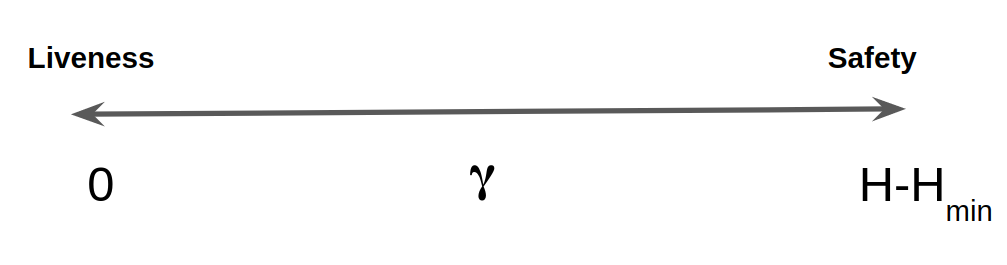
\includegraphics[width=0.6\columnwidth,
	keepaspectratio]{figures/gamma.png}
	\caption{The $\gamma$ parameter versus liveness and safety for either
	voting or activation.}
	\label{fig:gamma-parameter}
\end{figure}

This parametric definition of the threshold gives us the ability to adjust the
threshold based on the context of each individual proposal and not follow a one
size fits all approach. For example, for a very critical update we might
require a higher $\gamma$ value in order to ensure a greater safety for the
result by sacrificing some of the liveness and demanding a stronger consent
from the community.

Table \ref{table:threshold-examples} shows some examples of different threshold
functions $\tau(\gamma)$, expressed by means of the adversary stake ratio $r$,
$r = \frac{Adversary\ Stake}{Total\ Stake} = \frac{T}{T+H} = \frac{T}{100}$,
along with the corresponding constraint on $r$, derived from the $T < H_{min}$
constraint and $\frac{1}{r_{Th}}T < H_{min}$ constraint for voting and
activation respectively. The choice of $H_{min}$ recorded on the second column
determines the resulting threshold function, as well as the required constraint,
appearing in the respective columns. Our analysis is based on the assumption
that we can have an estimation of the adversary ratio $r$. From Garay et. al.
in~\cite{sok}, we know that the ratio $r$ is always upper bounded by the
theoretical adversary tolerance $r_{Th}$ of our consensus protocol, i.e.,
$r < r_{Th}$ (e.g., $r < 1/2 = r_{Th}$, or $r < 1/3 = r_{Th}$ etc.).

\begin{table}[h!]
	\centering
	\begin{tabular}{ | c | c | c | c |}
		\hline
		\textbf{Process} & $H_{min}$ & \makecell[c]{\textbf{Threshold}\\
		$\tau(\gamma) =
		H_{min} + \gamma$,\\ where $0 \leq \gamma < H-H_{min}$} &
		\makecell[c]{\textbf{Constraint}\\$T < H_{min}$ (for voting)\\
		$\frac{1}{r_{Th}T} < H_{min}$
		(for activation)} \\
		\hline
		\multirow{2}{*}{Voting} & $\frac{H}{2}$ &
		$50(1-r)+\gamma$ & $r < 1/3$
		 \\
		 & $T+1$ & $100r + 1 +\gamma$ & Any $r < r_{Th}$ \\
		\hline
		\multirow{2}{*}{Activation} & $\frac{H}{2}$ &
		$50(1-r)+\gamma$ &
		\makecell[c]{$r < \frac{r_{Th}}{2+r_{Th}}$ \\ ($r < 1/5$ for
		$r_{Th} = 1/2$)}
		\\
		 & $\frac{1}{r_{Th}}T + 1$ &
		$\frac{100r}{r_{Th}} + 1 + \gamma$ & Any $r < r_{Th}$ \\
		\hline
	\end{tabular}
	\caption{Examples of different threshold definitions.}
	\label{table:threshold-examples}
\end{table}

In table \ref{table:examples}, we provide examples of threshold values for
different values of
$\gamma$ and different adversary ratios r for a specific choice of the
$\tau(\gamma)$ function and a constraint relevant to the voting process. In
particular, for the function $\tau(\gamma) = H/2 + \gamma =
50(1-r)+\gamma$ and $r < 1/3$ (i.e., $H_{min} = \frac{H}{2}$ and $T <
\frac{H}{2}$). For a specific adversary ratio r, as we increase
$\gamma$, we require stronger honest stake majority, in order to avoid the
denial of approval attack, however this provides us with more safety. In this
particular case of $\tau(\gamma)$, the allowed
$\gamma$ values lie in the range $0 \leq \gamma <
H/2$. So in the table we have chosen the lowest possible
$\gamma$ value ($\gamma=0$), the maximum $\gamma$ value ($\gamma = \frac{H}{2} -
1$) (assuming for the sake of the example that
$\gamma$ takes integer values) and an intermediate value $\gamma = T$.

So for instance, in the line where $r=0.1$, we can see that the allowed range of
values for the threshold is $[45\%, 89\%]$. As long as the threshold is in this
range, we can have both liveness and safety (assuming $r=0.1$).We observe that
for low values of $\gamma$ ($\gamma = 0$), $H/2$ of honest stake is enough to
have liveness. In contrast, for high values of $\gamma$ ($\gamma = H/2 -1$), we
essentially require honest stake unanimity in order to have liveness.

\begin{table}[h!]
	\centering
	\begin{tabular}{ | c | c | c | c |}
		\hline
		Adversary ratio r ($r < 1/3 \approx 0.33$) & $\gamma = 0$ & $\gamma =
		T$ & $\gamma = \frac{H}{2} - 1$ \\
		\hline
		$0.1$ & $45\%$ & $55\%$ & $89\%$ \\
		$0.2$ & $40\%$ & $60\%$ & $79\%$ \\
		$0.3$ & $35\%$ & $65\%$ & $69\%$ \\
		\hline
	\end{tabular}
	\caption{Threshold values for different $\gamma$ and adversary
		ratios for a specific choice of $\tau(\gamma)$ ($\tau(\gamma) =
		50(1-r)+\gamma$), relevant to the voting
		process.}
	\label{table:examples}
\end{table}

\subsection{Ideation}
\label{sec:ideation}

The primary goal of the SIP is to capture the idea behind an update.
An SIP might contain
\begin{itemize}
\item title of the SIP,
\item hash of the SIP text,
\item author(s),
\item update justification,
\item update scope,
\item update constraints, e.g.:
  \begin{itemize}
  \item dependencies,
  \item conflicts w.r.t. other update proposals,
  \item prerequisites, etc.
  \end{itemize}
\item duration of the SIP voting period,
\item priority, etc.
\end{itemize}

Update proposals in this phase are recorded as a structured text document
(e.g., JSON format).
%
This design does not constrain where the SIP text is stored. A SIP that is
unavailable or whose hash does not match the one submitted on the chain can
simply be rejected by the community.

Update constraints, determine the feasibility of a system update.

The SIP is submitted to the blockchain by means of a fee-supported transaction.
Any stakeholder can submit an SIP, thereby proposing a system update.

The SIP submission takes place under a commit-reveal scheme, to ensure that the
ownership of the proposals is preserved.

Once the SIP is revealed, stakeholders can access all the its details and a
voting period starts. Note that stakeholders not only vote for the SIP, but also
for other characteristics of the update such as:
\begin{itemize}
\item type of change,
\item priority,
\item criticality, etc.
\end{itemize}
These characteristics are described in the SIP's metadata.

In the case that the evaluation of an SIP requires deep technical knowledge,
stakeholders can make use of a delegation mechanism which is described in
Section~\ref{sec:delegation-mechanics}.

\subsection{Implementation}
\label{sec:implementation}

During the implementation phase of an update, an SIP is implemented. This is an
off-chain process. Not all SIPs require an implementation. Examples of such SIP
include protocol-parameters updates, or fund transfers.

\subsection{Approval}
\label{sec:approval}

Once the implementation of an SIP is ready, the developer creates a bundle that
consists of:
\begin{itemize}
\item source code,
\item metadata,
\item and optionally binaries.
\end{itemize}
This bundle must be uploaded to a repository (decentralized or otherwise), and a
content-based hash must be produced to uniquely identify it. This hash, together
with other metadata, is called the \emph{update proposal} (UP). The UP is
submitted to the blockchain.

In addition to the data described above, protocol update proposals must specify:
\begin{itemize}
\item The version that they supersede. The update can only be applied to this
  version.
\item The (hash of the) proposal they supersede. Update proposals in the
  approval phase can have the same version, so proposals need to disambiguate
  the proposal they supersede. This allows us to avoid a situation in which a
  proposal depends on a given version, but also (implicitly) on a particular
  implementation of that version. If we do not make this dependency implicit,
  then we risk having an update being applied on the wrong version.
	%
	We cannot, on the other hand, enforce uniqueness of versions in update
  proposals, since we risk having malicious actors organizing a denial of
  service attack that prevents honest proposals from entering the system.
	%
	Note that having a proposal specify the proposal it supersedes require that we
  start with a Genesis (implementation) proposal.
\end{itemize}

This UP must be submitted to the blockchain for approval by the stakeholders to
move forward in the update process. Submission of the UP takes place using a
commit-reveal scheme.

All approved UPs are stored in the blockchain. This enables the developer to
find the appropriate source code version that will be updated (probably the
latest) using the link provided in the UP's metadata.

The review of the code requires advanced technical skills. For this reason we
expect the majority of stakeholders to make use of the delegation mechanism
describe in Section~\ref{sec:delegation-mechanics}.

The approval of a UP signifies the beginning of the \emph{activation} phase.

\subsection{Activation}
\label{sec:activation}

In the activation phase the protocol updates are \emph{activated}. Protocol
updates enter this phase after they are approved by the stakeholders.

The activation phase features an \emph{endorsement} period for signaled updates.
During this period the node operators can perform the manual steps necessary to
update the software. Once the software is installed, the update does not take
place right away, since the nodes need to synchronize to avoid chain splits. The
new protocol version remains in a latent state until activation takes place.

In a signaled update, the nodes use the endorsement period to signal other nodes
their readiness to run the new protocol version.

% Why not vote and endorse an implementation at the same time?
In this design it is important that an UP endorsement takes place \emph{after}
said UP gets approved.
%
This is because voting and endorsing in parallel:
\begin{itemize}
\item Constitutes a \emph{security risk}: malicious UPs can be easily deployed
  by encouraging the community to install a proposal before it is approved by
  the experts.
\item Undermines the authority of experts: the community would be less prone to
  follow the advice of a majority of experts if they can simply chose to install
  any submitted UP.
\item Favors community splitting: if two UPs that implement the same SIP are
  submitted, it would be unclear for the community which implementations they
  should download and install.
\end{itemize}

One popular method for signaling is to include the new version of the software
in the blocks the node issue. This denotes that they are ready to run the new
version. This is the approach taken by Bitcoin~\cite{bitcoin}. A drawback of
this method is that it restricts signaling only to \emph{block producing nodes},
thereby excluding other type of such as \emph{full-node clients},
\emph{light-node clients}, etc. A major drawback is that the activation of
changes is delayed by the block creation process which is slow.

An alternative signaling method that does not suffer from the drawbacks above is
to signal upgrade readiness by means of fee-based transactions. Such
transactions are bounded to stakeholder keys and therefore bound to specific
stake.
%
As a result we only have to wait for these messages to be stable on the
blockchain.

Furthermore, we could even use a separate consensus protocol, just for the
purpose to agree on the binary value carried by these messages (Ready | Not
Ready) (i.e., a binary Byzantine Agreement problem). The parties taking part in
this new protocol would be any node (client, or maintainer) that actively
participates in the underlying consensus protocol and thus needs to synchronize
with its peers with respect to the activation of some change. The main
assumptions (network, setup, computation as in Garay et al. \cite{sok}) of this
consensus protocol, naturally will be identical to the assumptions of the
underlying consensus protocol and therefore the
\emph{resiliency}\footnote{According to Garay et. al. in \cite{sok}, the
  resiliency is the fraction $(t/n)$ of misbehaving parties a protocol can
  tolerate, where $t$ are the number of adversaries and n are the total number
  of parties. In our case, we can assume that $t$ is the total adversary stake
  and $n$ is the total stake.} of the protocol will also be the same.

All in all, by departing from the block signaling solution, we can distinguish
between the readiness of different types of nodes and achieve a faster
calculation of the adoption threshold. Of course, the downsides in this case are
the added complexity and the extra fee that has to be paid for each activation
signal.

After a sufficient portion of the block producing nodes communicate that they
are able to run the new version the switch to the new protocol can take place.
This not happen right after such majority is reached, but instead the switch to
the new protocol version takes place at a predefined time in the future, most
likely the beginning of a new epoch.

The activation of non-signaled protocol updates do not require endorsements,
however their activation also takes place at a predefined time in the future.

\subsubsection{Secure activation of a new protocol version}
\label{sec:secure-activation-of-a-new-protocol-version}

A secure activation of a new version of the consensus protocol is one that
achieves a \emph{secure transition} from the current version to a new one. We
have formally defined what is a secure activation and have proposed two
distinct protocols that provably achieve this \cite{secure_activation}. In a
nutshell, secure activation means, the secure
transition
from the old ledger (L1) to the new ledger (L2) in a way where:
\begin{itemize}
\item L2 enjoys liveness \cite{backbone}
\item L2 enjoys consistency \cite{backbone}
\item L2 has L1 as a prefix
\end{itemize}
The first two properties ensure the security of the updated ledger while the
third property ensures the seamless continuation of the ledger history.

In \cite{secure_activation}, our first activation protocol requires the
structure of the current and the updated blockchain to be very similar (only
the structure of the blocks can be different) but it allows for an update
process more simple and efficient. The second activation protocol that we
propose is very generic (i.e., makes few assumptions on the similarities
between the structure of the current blockchain and the updated blockchain).
The drawback of this protocol is that it requires the new blockchain to be
resilient against a specific adversarial behavior and requires all the honest
parties to be online during the update process. However, we show how to get rid
of the latest requirement (the honest parties being online during the update)
in the case of proof-of-work and proof-of-stake ledgers. The interested reader
can find more details on this topic in our paper \cite{secure_activation}.

In Cardano, a specific protocol version is represented by a set of ledger rules
called \emph{an era}. The transition from one era to another takes place by a
module residing in the consensus layer named \emph{hard-fork combinator}. This
is the candidate module for implementing the proposed protocols in
\cite{secure_activation}. The hard-fork combinator is triggered by the update
system state in order to initiate the said transition.

\subsubsection{Overview of the activation process}
\label{sec:overview-of-the-activation-process}
When a protocol update proposal is approved\footnote{Cancellation and
	non-protocol update proposals come into effect immediately after being
	approved.} it enters a \emph{priority queue} where it waits to be activated.
The priority is determined by the update proposal's versions. A
proposal with lower version will activate \textbf{before} a proposal with a
higher version.
%
We call the proposals in the activation queue the \emph{approved proposals}.

Proposals \textbf{must increase} the current \emph{protocol-version} that the
chain supports. The protocol version consists of two components:
\begin{enumerate}
	\item The major version, which is used to specify hard-forks.
	\item The minor version, which is used to specify soft-forks.
\end{enumerate}
Protocol-versions of update proposals do not need to be unique.

The update system guarantees that the protocol versions can only strictly
increase. In this way, the update system can rely on the update proposal's
protocol-version and its declared predecessor version to:
\begin{itemize}
	\item Determine priorities: a lower version (higher priority) is activated
	before a higher version (lower priority) one; specifying the version gives
	us
	a simple way to specify urgency.
	\item Resolve conflicts: a proposal declares \textbf{one and only one}
	version
	that it supersedes (its predecessor). Thus a proposal is in conflict with
	all
	others except the one that it supersedes.
	\item Check dependencies: a proposal depends only on the one it supersedes.
\end{itemize}
This design decision requires:
\begin{itemize}
	\item The implementers to pick exactly one version their update is
	compatible
	with, and determine which version their update should determine.
	\item The experts to check the version that an update has, and the
	compatibility
	with the version it supersedes.
\end{itemize}

The protocol-versions of the proposals in the activation phase are unique. If a
proposal is approved it enters the activation phase. If its protocol version
corresponds to a proposal already in the activation phase, then the old proposal
is canceled (see Section~\ref{sec:cancellations} which deals with
cancellations). In the unlikely case that two approved proposals:
\begin{enumerate}
	\item have the same voting period end, and
	\item update to the same protocol version
\end{enumerate}
we resolve this conflict by:
\begin{enumerate}
	\item picking the proposal with the highest stake in favor, or
	\item picking the proposal with the greatest hash, if they have the same
	stake
	in favor.
\end{enumerate}

The approved proposal at the front of the activation queue will enter the
\emph{endorsement period} if it supersedes the current version (see
Section~\ref{sec:entering-the-endorsement-phase}).
%
There can be \emph{at most one protocol update proposal} in the endorsement
period at any time.
%
This is to avoid the stake of the stakeholders being split among competing
proposals during endorsement, and thus, when changes take effect.
%
We call a proposal that is in the endorsement period the \emph{candidate
	proposal}.

If the new candidate proposal is a signaled protocol-update, the block producers
can start \emph{endorsing} it.
%
If the proposal gathers enough endorsements, then it can be
\emph{scheduled-for-activation}.

If the candidate proposal is a non-signaled protocol update, e.g. it is a
parameters update, it becomes scheduled at $2k$ slots before the end of an
epoch, where $k$ is maximum \emph{number of blocks} the chain can roll back (see
Section~\ref{sec:on-cutoff-points-for-endorsements}).

A scheduled proposal \textbf{waits} to be activated \textbf{till the first slot
	of the next epoch}. In case of non-protocol updates, the proposal does not
need to be activated. The ledger simply records its approval and might decide to
update the state in any way it sees fit (for instance by transferring funds
either right away or at the beginning of a new epoch).

The next sub-sections describe the details of the activation protocol outlined
above.

\subsubsection{Entering the endorsement period}
\label{sec:entering-the-endorsement-phase}

An update proposal can enter the endorsement period if two conditions are met:
\begin{enumerate}
	\item It is at the front of the priority queue (i.e. it is has the lowest
	version among the proposals queue).
	\item The version and proposal hash that the proposal declares to supersede
	must
	be \textbf{the same} as the current version.
\end{enumerate}
Once in the endorsement period, \textbf{it might return to the queue} if a new
update proposal is approved and ends up in front of the priority queue (which
means that the newly approved proposal has a lower version than the current
candidate).

\subsubsection{Endorsements of signaled protocol updates}
\label{sec:endorsemnts}

Only signaled protocol updates need endorsements, since they require nodes to
download and install new software, and signal that they are ready to run the new
version.
%
These kind of update proposals have a \emph{safety lag} associated with them,
which is a time window that ensures sufficient time is provided to the parties
to download and deploy a candidate proposal.
%
This safety lag determines the duration of the endorsement period and
\textbf{must be specified in number of epochs}. As a result, the end of the
safety lag coincides with the end of an epoch.

When a signaled protocol-update proposal becomes a candidate, block producers
can start endorsing it. The stake associated with the keys endorsing the
proposal is tallied $2k$ blocks before the end of an epoch. We consider the
stake \textbf{at the slot in which we tally}. We have two activation thresholds
depending on the epoch in which the tally takes place:
\begin{itemize}
	\item If the next epoch does not coincides with the end of the safety lag,
	then
	this threshold is the \emph{adoption threshold} ($\tau_A$).
	\item If the next epoch coincides with the end of the safety lag, then this
	threshold is set to $51\%$.
\end{itemize}

Once we sum up the stake endorsing a proposal there are three possibilities:
\begin{enumerate}
	\item If the proposal has not gathered enough endorsing stake then:
	\begin{enumerate}
		\item If the safety lag expires on the next epoch then the proposal is
		canceled.
		\item If the safety lag does not expire on the next epoch then the
		proposal
		can continue to be endorsed on the next epoch. The endorsements are
		carried
		over.
	\end{enumerate}
	\item If the proposal has gathered enough endorsing stake, then it is
	\emph{scheduled for activation} at the beginning of the next epoch.
\end{enumerate}

Protocol updates (signaled and otherwise) get activated \emph{at the beginning
	of an epoch}. The reason for this is that the ledger and consensus rules
	rely
on these to be stable during any given epoch.

The cancellation\footnote{Note that we classify expired proposals, i.e.
	proposals that did not get enough endorsements at the end of the safety lag,
	as canceled proposals.} or activation of a proposal causes its removal from
the activation queue, and the next implemented proposal in the queue that
supersedes the current protocol version, if any, to become the new candidate and
enter the endorsement period.

A proposal being endorsed can go back to the queue (see
Section~\ref{sec:the-queue}). In this case the endorsements for this proposal
are discarded.

\subsubsection{Parameters update}
\label{sec:parameters-update}

Parameters-updates proposals are special kind of non-signaled protocol updates.
They determine new values for the (existing) protocol parameters. The current
version of the software should be able to deal with this sort of updates.
Therefore there is no need for the nodes to download and install software, and
thus no need for an endorsement period. However, they can only be activated at
beginning of an epoch. Parameters-update must also wait in the activation queue.

A protocol parameters update must have a corresponding approved SIP, which
justifies the need for changing the parameter values. The submitted
implementation (UP) specifies the new values and the new protocol version
associated to these parameters. Both SIP and UP describe the parameters change.
The SIP does this in an abstract way, e.g. ``change maximum block size to 1MB'',
whereas the UP describes this change in a concrete way, e.g.
\texttt{maxBlokcSize = 1024}.

Note how, unlike Byron, the activation of one parameter update does not
automatically eliminate all the other pending parameters updates. We rely on the
versioning scheme for resolving conflicts. For instance, assume the current
protocol version is \texttt{1.0.0}. If updates with versions \texttt{1.1.0} and
\texttt{1.2.0} both change a parameter \texttt{p}, activating \texttt{1.1.0}
does not necessarily causes \texttt{1.2.0} to be discarded. It all depends on
the version the \texttt{1.2.0} supersedes. If it supersedes \texttt{1.0.0}, then
it will be canceled since the current version is now \texttt{1.1.0} and versions
can only increase. However \texttt{1.2.0} could declare that it supersedes
version \texttt{1.1.0}, in which case it can be activated after this version
(for instance in the next epoch).

\subsubsection{Non-protocol updates}
\label{sec:non-protocol-updates}

Non-protocol updates do not change neither the consensus rules nor the ledger
rules that the blockchain nodes execute. Therefore the do not enter the
activation phase.
%
When this kind of updates are approved, the update system simply records this
event,
and it is the ledger responsibility to react accordingly. For instance, if the
update concern funds transfers from the treasury, then the ledger must update
its state by performing the transfer described in the update.

If the update concerns an application that uses the blockchain (e.g. a wallet),
then the dependencies between this application and protocol that the blockchain
runs managed off-chain.
%
Such dependency management is the responsibility of developers (who implement
the updates) and experts.
%
The update system can provide metadata for specifying the dependencies and/or
conflicts of an application with the rest of the ecosystem, but the update
system will not check this.

Just like with the other kind of updates, non-protocol updates must have a
corresponding approved SIP and implementation.

\subsubsection{Explicit cancellation}
\label{sec:explicit-cancellation}

A proposal can be explicitly canceled. This allows the experts and community to
cancel an approved implementation after a (significant) problem with it was
discovered.

An explicit cancellation is submitted as a SIP that must justify the reason for
canceling the proposals. When submitted as an update proposal (UP), the
cancellation must specify the proposals that it will cancel if approved.

The explicit cancellation also goes through the ideation and approval phases,
however, the explicit cancellation \emph{immediately cancels} the proposals it
refers to once it gets approved by the expert pools in the approval phase.

Cancellation proposals have no next-versions associated with it. They only
specify the hash of the implementations they cancel.

\subsubsection{Cancellations}
\label{sec:cancellations}

There are several factors that can cause a proposal to be canceled:

\begin{itemize}
	\item The proposal is explicitly canceled by a cancellation proposal that
	made
	it past the approval phase.
	\item The proposal is overridden by another proposal with the same version
	that
	made it through the approval phase. If the experts approve such proposal,
	then
	this gives a strong indication that the older proposal should be discarded.
	%
	Note that even though the system guarantees that only one proposal
	per-version
	will get approved in any given slot (as described earlier), there might be
	proposals approved with the same version as a proposal approved in a
	previous
	slot.
	\item The proposal supersedes a version that can never follow. Protocol
	versions
	increase monotonically. So if an update depends on a version that is lower
	than the current version we know for sure that such version can never be
	seen
	on the chain, and therefore the proposal that depends on this version can be
	discarded.
\end{itemize}

If the candidate proposal already got the required endorsements (which means
that the cancellation arrived at or later than the slot at which the tally
occurred, this is $2k$ blocks before the end of an epoch), and is waiting to
be activated, then the cancellation update cannot stop it. In this case, a new
software update must be implemented and submitted that will correct the
identified problem.

If a candidate proposal is non-signaled, but the cancellation arrives
\textbf{after} $2k$ blocks before the end of the epoch, then it cannot be
canceled either for the reasons given in
Section~\ref{sec:on-cutoff-points-for-endorsements}.

Nodes that upgraded to a canceled version can continue to operate normally
following the current version since the upgraded version \textbf{must} be able
to follow the current ledger and consensus rules.
%
Then it is up to the node operators to revert back to the previous version, or
continue using the software version that can also validate the protocol version
that got discarded. The ledger rules \textbf{shall ensure} that this discarded
protocol version is never applied.

\subsubsection{The queue}
\label{sec:the-queue}

Approved proposals enter an activation priority queue. The order of the queue is
determined by the proposals' versions. This queue \textbf{shall not} contain any
duplicated versions. If a proposal with the same version as a proposal from the
queue gets approved, then:

\begin{enumerate}
	\item If the old proposal (the one in the queue\footnote{Note that only the
		proposal in front of the queue can receive endorsements.}) does not have
	enough endorsements by the time the new proposal is approved, then the old
	proposal is canceled.
	\item If the old proposal has enough endorsements, then the new proposal is
	canceled.
\end{enumerate}

If a proposal with a lower version than the current candidate enters the queue
(i.e. the front of the queue changes), then we also have two situations:

\begin{enumerate}
	\item If the candidate proposal does not have enough endorsements, then it
	is
	put back in the queue, and the new proposal enters the queue.
	%
	If this new candidate gets eventually approved then the old proposal will be
	canceled (since it will supersede a version lower than the current version).
	%
	However, since it is possible that the new proposal gets canceled (for
	instance due to lack of enough endorsements), we leave the old proposal in
	the
	queue.
	\item If the candidate proposal has enough endorsements, then the new
	proposal
	gets discarded (since it will be superseding an older version that will
	never
	be adopted since versions increase monotonically).
\end{enumerate}

\subsubsection{Cut-off points for endorsements}
\label{sec:on-cutoff-points-for-endorsements}

The ledger layer must provide future information about a part of its state. In
particular, it should be able to tell up to $k$ blocks in the future if a new
protocol version will be activated. To this end, we require that the \emph{last
	endorsement} required for meeting the adoption threshold \emph{is stable}
	$k$
blocks before the end of the epoch. This means that endorsements for a given
proposal for a given epoch are considered up to $2k$ blocks before the end of
that epoch. This is not to say that the endorsements after this cut-off point
will not be considered, they will in the next epoch.

To see why this is required, consider a last endorsement (required to meet the
threshold) arriving between $2k$ blocks and $k$ blocks before the end of an
epoch, which will happen at block number $b_e$. If the ledger is asked between
blocks $b_e - k$ and $b_e$ whether a new version will be activated at $b_e$, the
answer depends on the stability of the last endorsement. If it is not stable,
then replying ``yes'' might be incorrect, since we can roll back and switch to a
fork where that endorsement never occurred. If we reply ``no'', then this might
also be incorrect if we continue in that fork.

\subsection{When multiple client implementations exist}

In the cases where the consensus protocol is open, alternative client
implementations might exist (for instance in different languages and/or different
licensing schemes).
%
As we have seen, our mechanism has a separate on-chain voting phase during the
ideation phase (Section~\ref{sec:ideation}).
%
In this phase a formal-spec/design of the protocol update is submitted (as an
SIP).
%
So the update mechanism defined in this document \emph{clearly distinguishes
  the protocol update decision from the implementation approval decision}.
%
The latter takes place in the second on-chain voting phase, the approval phase
(Section~\ref{sec:approval}), which references the approved SIP.

In a multi-implementation setting, what the community really needs to approve
and endorse is the protocol upgrade, and not a particular implementation per se.
%
The implementation adopted by each participant in the network is something that
cannot be controlled.
%
However, in the approval phase mentioned above, we can still have a ``blessed''
\emph{reference implementation} of the upgraded protocol, or even have a single
proposal that includes multiple implementations (e.g., in different languages)
that are approved/blessed by the community.

\section{Performance analysis}
\label{sec:performance-analysis}

\subsection{Impact on transaction throughput}
\label{sec:impact-trans-thro}

An important measurement of a blockchain system's performance is the number of
transaction bytes per-second ($\mathit{TBPS}$) it can sustain. Unlike the more
commonly used metric, transactions per-second, this number is not dependent on
the chosen size of a transaction (which would allow to manipulate it at will by
choosing different transactions sizes). Running an update mechanism on the
blockchain should not result in a substantial performance degradation.
Therefore, in this section we estimate the impact on performance that the
proposed update mechanism will have on a system's TBPS. Our estimations are
based on \emph{worst case scenarios}, which allow us to determine upper bounds
for the performance impact of the update mechanism.

Given a payload size in bytes ($\mathit{psize}$) that needs to be stored in a
blockchain, the blockchain's throughput measured in $\mathit{TBPS}$, and the
duration of the update process ($\mathit{duration}_u$), we can calculate the
percentage of the system's $\mathit{TBPS}$ ($\mathit{usage}_{\mathit{pct}}$) that
will be used by the update payload as follows:
$$\mathit{usage}_{\mathit{pct}} = 100\frac{\mathit{psize}}{\mathit{TBPS} ~
\mathit{duration}_u}$$

An update consists of several phases (ideation, implementation, approval, and
activation). In each phase, there are three types of messages being sent:
commits, reveals, and votes.

% Why do we consider only the voting period:
Before the voting phases, where votes can be cast by the participants, each
update requires only two messages spread across two stability windows, needed
for transactions to stabilize in the chain. These stability windows are quite
large, e.g. in Cardano the stability window is 1 day and a half. As a result,
only two messages need to be transmitted for the commit-reveal phase over a
large period of time, which means that a blockchain system can easily handle
this. This leaves us with the voting phase as the sole source for performance
degradation that can be caused by the update mechanism.

% Why do we consider phases in isolation
In addition, note that we only need to consider the additional load introduced
by the update mechanism during a single phase. It is in the voting period of
each phase where the system should be able to handle the additional load, since
the update mechanism introduces very little load between voting phases.

We define the worst-case scenario for a voting period in terms of
\begin{itemize}
\item number of participants ($n_p$), e.g. voters (note that in the worst case
  scenario everybody will vote, regardless of their stake, which means that the
  stake distribution is irrelevant for this analysis)
\item number of update proposals being voted at the same time ($n_c$), during
  the same period (note that in the worst case scenario multiple update
  proposals will coincide in the start and end of the voting period, otherwise
  the system would have a larger time interval to distribute the load).
\item number of time a participant changes her vote ($n_r$), per-update proposal
\end{itemize}
Then, we can calculate the worst case scenario for the number of bytes that need
to be transmitted as part of the vote payload ($\mathit{psize}_v$) as:
$$\mathit{psize}_v = s_v \mathit{n_p} n_r n_c$$

The size in bytes for $s_v$ was obtained by calculating the size CBOR
encoding~\cite{RFC7049} of the vote payload of our prototype. This payload
includes:
\begin{itemize}
\item The hash of the voted SIP. We use 32 bytes hashes, so considering the 1
  byte CBOR tag this gives us a total 33 bytes.
\item The confidence (for, against, abstain), which can be encoded in 1 byte
  (which also included the CBOR tag).
\item The key of the voter. We use 32 bytes keys, so this give us a total of 33
  bytes, when we consider the CBOR tag.
\item The vote signature. We consider 64 bytes signatures, which are accompanied
  by a 32 bytes key. This results in 64 + 32 + 1 bytes required for the
  signature.
\end{itemize}
So a vote requires in total 164 bytes.

Table~\ref{fig:tab:worst-case-analysis-voting-period} shows the results of the
worst case analysis for different parameter values, where $\mathit{duration}_v$
is the number of voting days, which was used to calculate the voting period
duration. For this analysis we use the $\mathit{TBPS}$ that Cardano currently
achieves in mainnet: $3.2$ Kb/s. This number is obtained from dividing the
maximum block body size, $64$ Kb, by the number of seconds per-block, $20$.

\begin{table}[!htb]
	\centering
	% NOTE: DO NOT EDIT THE TABLE BELOW: It was generated by the
	% 'worst-case-analysis' benchmark, which can be found in the
	% `input-output-hk/decentralized-software-updates/formal-spec/bench`
	% directory (github).
  \begin{tabular}{| r | r | r | r | r |}
    \hline
    $n_p$ & $n_r$ & $n_c$ & $\mathit{duration_v}$ & $\mathit{usage_{pct}}$\\
    \hline
    1000 & 2 & 1 & 7 & 0.017\\
    1000 & 2 & 5 & 7 & 0.083\\
    1000 & 2 & 10 & 7 & 0.166\\
    10000 & 2 & 1 & 7 & 0.166\\
    10000 & 2 & 5 & 7 & 0.828\\
    10000 & 2 & 10 & 7 & 1.655\\
    100000 & 2 & 1 & 7 & 1.655\\
    100000 & 2 & 5 & 7 & 8.277\\
    100000 & 2 & 10 & 7 & 16.555\\
    1000000 & 2 & 1 & 7 & 16.555\\
    1000000 & 2 & 5 & 7 & 82.773\\
    1000000 & 2 & 10 & 7 & 165.546\\
    1000000 & 2 & 10 & 14 & 82.773\\
    1000000 & 2 & 10 & 30 & 38.627\\
    10000000 & 2 & 1 & 7 & 165.546\\
    10000000 & 2 & 5 & 7 & 827.729\\
    10000000 & 2 & 10 & 7 & 1655.458\\
    \hline
  \end{tabular}
	\caption{Worst-case analysis TBPS	for a voting period}
	\label{fig:tab:worst-case-analysis-voting-period}
\end{table}

Figure~\ref{fig:usage-vs-participants} shows the worst case usage as a function
of the number of participants, assuming 10 concurrent update proposals, a 7 day
voting period, and each participant changing her vote twice.

\begin{figure}[!htp]
	\centering
	% NOTE: DO NOT EDIT THE PICTURE BELOW: It was generated by the
	% 'worst-case-analysis' benchmark.
  \begin{tikzpicture}
    \begin{axis}[
      title={Participants vs usage percentage},
      xlabel={Participants},
      xmode=linear,
      ylabel={Usage percentage},
      ymode=linear,
      ytick={0, 20, 50, 100, 150, 200},
      legend pos=north west,
      ymajorgrids=true,
      grid style=dashed,
      ]
      \addplot[color=black] table {data/participants-vs-usage.dat};
    \end{axis}
  \end{tikzpicture}
	\caption{Worst case scenario analysis for system's usage with 10 concurrent
	update proposals}
	\label{fig:usage-vs-participants}
\end{figure}

Looking at Table~\ref{fig:tab:worst-case-analysis-voting-period} and
Figure~\ref{fig:usage-vs-participants}, we can see that the usage percentage
scales linearly in the number of participants\footnote{Note the logarithmic
  scale used in Figure~\ref{fig:usage-vs-participants}}, i.e., a 10 times
increase in the number of participants will increase 10 times the required usage
percent.
%
We can see that the impact of the update protocol on the
system's performance is negligible up to $100,000$ participants and $1$ proposal
being voted.

However, in spite of the usage percentage being a linear function of the number
of participants, when we pass the million participants or $100,000$
participants vote on $10$ proposals at the same time, we start seeing a
considerable impact of the update protocol on the system's performance.
%
In case $1$ million participants would vote on $10$ proposals at the same time,
the system could not process the extra payload. Nevertheless, this would require
that the worst case conditions we assume in this analysis being met: $10$ SIP's
being voted at the same time over the period of $7$ days, where each participant
votes twice. In practice we will have a much higher voting duration, and not all
proposals will overlap exactly in their voting period, which means that the
additional payload can be spread across a much larger time interval.

There are several alternatives to allow a blockchain system to accommodate more
participants or concurrent update proposals:
\begin{itemize}
\item Use of expert pools. By having the participants delegate their voting
  rights, the number of voters can be substantially reduced, while increasing
  voter's turnout.
\item Increase in the duration of the voting period. We have used a very short
  voting duration (7 days). In practice update proposals would require that
  voters are given a much longer time to decide, specially if the update
  proposal has a large impact on the network.
\item Increase the maximum block size that the protocol allows, which will
  result in a larger TBPS. Note also that the current maximum block size in the
  Cardano protocol, which we use for our worst case analysis, is quite small but
  sufficient for accommodating the blockchain current usage. If the blockchain
  would need to process additional payload, experiments show that Cardano can
  increase its maximum block size up to $1$Mb, which would result in a tenfold
  increase in the TBPS, and therefore a tenfold increase in the number of
  participants that the update protocol can accommodate.
\end{itemize}

The back-of-the-envelope calculation described in this section was put to the
test against the data generated by actual runs of the update protocol on a
testnet. We present next the setup of our experiments and the results we obtained.

Our goal was to measure the impact of the voting process on the blockchain's
transaction throughput. To this end, we fixed the protocol parameters of the
network, and ran experiments in which we gradually increased the number of
participants that voted on a proposal.

We used the testnet setup described in Section~\ref{sec:impl-this-design},
which consisted of 10 nodes running a stake pool each. The nodes were deployed
on AWS machines, distributed across 4 countries and 3 continents.

The protocol parameters were chosen in such a way that they resembled the
mainnet conditions, while allowing us to run experiments in a reasonable amount
of time. This means that in our testnet:
\begin{itemize}
\item like the Cardano network, blocks were produced every 20 seconds.
\item unlike the Cardano network, the stability window was set to 30 minutes
  (in Cardano this is 36 hours).
\end{itemize}
Using these parameters we could run each experiment in about 2 hours, depending
on the number of voters, since more voters required more time to register
staking keys, which we used as voting keys.

In each node that ran a stake pool (pool node) we ran:
\begin{itemize}
\item 50 threads that were constantly submitting UTxO transactions to the
  network.
\item a varying number of threads that submitted the votes on a given SIP
  proposal.
\end{itemize}

Each experiment carried out the following steps:

\begin{enumerate}
\item Start the UTxO transaction submission threads.
\item Register stake keys that will be used to vote on the SIP.
\item Submit an SIP commit, wait for it to become stable on the chain, and then
  reveal the SIP.
\item Wait for the voting period for the submitted SIP to open and then have
  all the participants in all the nodes vote in parallel.
\item After all participants voted, check that the number of voters matched the
  expected number of participants to make sure that each vote went through.
\end{enumerate}

After running the experiment we analyzed the script and node logs to count the
number of UTxO transactions that were submitted during the voting period.
Table~\ref{tab:experimental-results-tps} shows the results we obtained, and
this information is also plotted on Figure~\ref{fig:experimental-results-tps}.

\begin{table}[!htb]
  \centering
  \begin{tabular}{| r | r | r | }
    \hline
    Voters per node & TPS & Usage \% \\
    \hline
    1    & 16.64764543 & 0.036  \\
    10   & 16.5933518  & 0.362  \\
    100  & 16.04376731 & 3.662  \\
    250  & 15.14626039 & 9.051  \\
    500  & 13.64155125 & 18.087 \\
    750  & 12.13795014 & 27.115 \\
    1000 & 10.63822715 & 36.121 \\
    1250 & 9.127977839 & 45.189 \\
    \hline
  \end{tabular}
  \caption{Experimental results on TPS}
  \label{tab:experimental-results-tps}
\end{table}

\begin{figure}[!htb]
  \centering
  \begin{minipage}{0.45\linewidth}
  \begin{tikzpicture}
    \begin{axis}[
      title={Participants vs TPS},
      xlabel={Participants per node},
      xmode=linear,
      ylabel={TPS},
      ymode=linear,
      legend pos=north west,
      ymajorgrids=true,
      grid style=dashed,
      ]
      \addplot[color=black] table {data/participants-vs-tps.dat};
    \end{axis}
  \end{tikzpicture}
  \end{minipage}\hfill
  \begin{minipage}{0.45\linewidth}
  \begin{tikzpicture}
    \begin{axis}[
      title={Participants vs Usage \%},
      xlabel={Participants per node},
      xmode=linear,
      ylabel={Usage \%},
      ymode=linear,
      legend pos=north west,
      ymajorgrids=true,
      grid style=dashed,
      ]
      \addplot[color=black] table {data/participants-vs-usage-benchmarks.dat};
    \end{axis}
  \end{tikzpicture}
  \end{minipage}
  \caption{Experimental results on TPS}
  \label{fig:experimental-results-tps}
\end{figure}

The results shown in Table~\ref{tab:experimental-results-tps} coincide with our
back-of-the-envelope calculation regarding the impact of the voting phase on
the transaction throughput. We can observe a linear relationship between TPS
(or equivalently usage) and number of participants.

\subsection{Impact on latency}
\label{sec:impact-latency}

Addionally to the throughput, in our testnet experiments, we have measured the
impact on the \emph{transaction latency}. By ``latency'', we mean the
\emph{average end-to-end time} from the transaction submission until it appears
in the ledger. To this end, we have used the same setup as in the throughput
experiments: a 10 node geographically distributed network, where $50$ threads
per node constantly submit transactions and we utilize a varying number of
voters that try to vote in a $30$ minute voting period window.

In table \ref{tab:experimental-results-latency}, we record our main results.
Initially, with a single voter per node and as we are submitting transactions
almost at maximum capacity, we observed an average latency of around $25$
seconds. Then,
as we gradually increase the number of voters, we observe the latency
increasing. In the rightmost column of table
\ref{tab:experimental-results-latency}, we have recorded the factor by which
this latency-increase takes place for each increase of the voters load. In
figure \ref{fig:experimental-results-latency}, we observe a quadratic
increase of the latency with the increase of the load. Note that  when the
voting period is open, all participants vote at the same time. As a consequence
a queue is formed which causes the latency to increase. The size of this queue
will be dependent on the number of participants. Clearly, all participants
voting at the
same time is unrealistic, but even in this extreme situation we can accommodate
a large number of votes ($12500$) in $30$ minutes. Moreover, apart from the
simultaneous voting, a more realistic voting duration (e.g., of some days, or
weeks) would make the latency even more tolerant to the increase of the load.

\begin{table}[!htb]
	\centering
	\begin{tabular}{| r | r | r |}
		\hline
		Voters per node & (Average) Latency (sec) & Times increase \\
		\hline
		1    & 25.90 & 1\\
		10   & 25.88 & 1 \\
		100  & 25.36 & 1 \\
		250  & 46.73 & 1.8 \\
		500  & 105.99 & 4.1\\
		750  & 214.54 & 8.3\\
		1000 & 397.76 & 15.3\\
		1250 & 692.38 & 26.7\\
		\hline
	\end{tabular}
	\caption{Experimental results on Latency}
	\label{tab:experimental-results-latency}
\end{table}

\begin{figure}[!htb]
	\centering
	\begin{minipage}{0.45\linewidth}
		\begin{tikzpicture}
			\begin{axis}[
				title={Participants vs Latency},
				xlabel={Participants per node},
				xmode=linear,
				ylabel={Latency(sec)},
				ymode=linear,
				legend pos=north west,
				ymajorgrids=true,
				grid style=dashed,
				]
				\addplot[color=black] table {data/participants-vs-latency.dat};
			\end{axis}
		\end{tikzpicture}
	\end{minipage}\hfill
	\caption{Experimental results on Latency}
	\label{fig:experimental-results-latency}
\end{figure}

\subsection{Impact on processing time}
\label{sec:impact-proc-time}

Clearly the most processing intensive task of the update mechanism
is the tally phase. It is the phase where all the collected votes
are counted in order to reach a decision for a specific proposal.

We start with a theoretical time complexity analysis where we
assume a worst-case scenario, where we have $n$ participants that all
of them vote by submitting a single vote. Also we assume that we have
a single proposal, so that within a voting period, the number $n$ of
participants coincides to the number of submitted votes.

In the following, we try to break up the operations during the tally phase. In
the heart of the tally phase lies the following function call, which is called
for each proposal.

\definecolor{uppercasecolor}{rgb}{0.4,0,0.6}

\lstdefinelanguage{PriviHaskell}
{ basicstyle=\ttfamily\small,
  keywordstyle=[2]{\ttfamily\color{uppercasecolor}},
  morekeywords={class, do, type, forall},
  morekeywords=[2]{Commit, Hash, Int, VKeyHash, Proposal, SIP, E,
    StablySubmitted, Revealed, Submitted, Just, Either,
    Trace, State, Tick, Submit, Reveal,
    Valid, Invalid,
    UpdateSpec, SpecId, Submission, Revelation, MockSIP, MockImpl,
    UpdateEvent, E, UpdateState, TraceFragment, UpdateSUT,
    Is, Rejected, WithNoQuorum, Expired, Approved, Undecided, Queued,
    ActivationExpired, ActivationCanceled, ActivationUnsupported,
    BeingEndorsed, Scheduled, StablyRevealed, Activated,
    Unknown
  },
  sensitive=true,
  morecomment=[l]{--},
  morestring=[b]",
  literate=
    {->}{{$\rightarrow\;$}}1
    {=>}{{$\Rightarrow\;$}}1
    {=>}{{$\Rightarrow\;$}}1
    {++}{{\code{++}}}1
    {~}{{\ }}1
    {\\dollar}{{$\$$\;}}1
    {\\}{{$\lambda\;$}}1
    {/=!}{{$\neq\;$}}1
    {<!}{{$<\;$}}1
    {||!}{{$\vee\;$}}1
    {not}{{$\neg\;$}}1
}
\lstnewenvironment{haskell}{\lstset{language=PriviHaskell}}{}
\newcommand{\hinline}[1]{\lstinline[language=PriviHaskell]{#1}}

\begin{lstlisting}[language=PriviHaskell, caption=Tally phase initial function call]
	tallyStake confidence result ballot stakeDistribution adversarialStakeRatio
	=
	if stakeThreshold adversarialStakeRatio (totalStake stakeDistribution)
	<
	stakeOfKeys votingKeys stakeDistribution
	then Just result
	else Nothing
	where
	votingKeys = Map.filter (== confidence) ballot
\end{lstlisting}

Function \hinline{stakeThreshold} is constant whereas \hinline{Map.filter}
\footnote{\href{url}{http://hackage.haskell.org/package/containers-0.6.2.1/docs/Data-Map-Strict.html\#g:25}},
is $O(n)$ so \hinline{votingKeys} is $O(n)$, where $n$ is the number of
votes, which as we have said coincides to the number of participants. At this
point, we have a single pass (loop) over $n$ votes.

The remaining function used in the definition of \hinline{tallyStake},
\hinline{stakeOfKeys}, calculates the stake associated to the given key-map,
and is defined as follows:
\begin{lstlisting}[language=PriviHaskell, caption=Counting voting stake]
	stakeOfKeys keyMap StakeDistribution { stakeMap }
	= Map.foldl (+) 0 (stakeMap `Map.intersection` keyMap)
\end{lstlisting}
The $intersection$ function in the worst-case is
$O(n)$\footnote{\href{url}{http://hackage.haskell.org/package/containers-0.6.2.1/docs/Data-Map-Strict.html\#v:intersection}}.
Therefore this is a second pass (loop) over the data of length $n$. Finally, we
call \hinline{foldl} with a constant time operation, \hinline{+}, which
means that this call is also
$O(n)$\footnote{\href{url}{http://hackage.haskell.org/package/containers-0.6.2.1/docs/Data-Map-Strict.html\#v:foldl}}.
This is a third pass (loop) over the data of length $n$. Thus from the above
analysis we see that we have for a single proposal a call of
\hinline{tallyStake}, where in each such call we have three passes over the
data of length $n$. So in total for a single proposal we do $3$ passes over the
data of length $n$. That is $3n$ operations, which means that the tally time
complexity is $O(n)$.

This result is also confirmed by the experimental evaluation shown in
Figure~\ref{fig:eltime-vs-participants}, where we see that the processing time
increases linearly with the number of participants. In addition, we see that it
takes almost one tenth of a second to process the votes of $1$ million
participants. These results correspond to a single-core execution of the tally
algorithm on a i7 CPU laptop with 32GB of RAM.

\begin{figure}[!htp]
	\centering

	\begin{tikzpicture}
		\begin{axis}[
			title={Processing time (sec) vs Number of participants},
			xlabel={Participants},
			xmin=100.0,
			xmax=1.0e7,
			xmode=log,
			xtick={10.0, 100.0, 1000.0, 10000.0, 100000.0, 1000000.0, 1.0e7},
			ylabel={Processing time (sec)},
			ymin=0.0000001,
			ymax=10,
			ymode=log,
			ytick={0.0000001, 0.000001, 0.00001, 0.0001, 0.001, 0.01, 0.1, 1,
			10},
			legend pos=north west,
			ymajorgrids=true,
			grid style=dashed,
			]
			\addplot[color=black] table
			{data/participants-vs-elapsed_time.dat};
		\end{axis}
	\end{tikzpicture}

	\caption{Worst case scenario analysis for tally phase processing time}
	\label{fig:eltime-vs-participants}
\end{figure}

\subsection{Low impact on memory consumption}
\label{sec:low-impact-memory}

Finally, we present the measurements of the memory consumption during the tally
phase. As the graph in Figure \ref{fig:memcons-vs-participants} shows, the
memory allocated scales linearly in the number of participants. Moreover, our
measurements show that the allocated memory essentially corresponds to the space
required for storing the $256$ bit hashes of the public keys of the participants
in a Haskell map\footnote{\href{url}{http://hackage.haskell.org/package/containers-0.6.2.1/docs/Data-Map-Strict.html}}.

\begin{figure}[!htp]
	\centering

	\begin{tikzpicture}
		\begin{axis}[
			title={Memory consumed (MBs) vs Number of participants},
			xlabel={Participants},
			xmin=100.0,
			xmax=1.0e7,
			xmode=log,
			xtick={10.0, 100.0, 1000.0, 10000.0, 100000.0, 1000000.0, 1.0e7},
			ylabel={Memory consumed (MBs)},
			ymin=1,
			ymax=10000,
			ymode=log,
			ytick={1, 10, 100, 1000, 10000},
			legend pos=north west,
			ymajorgrids=true,
			grid style=dashed,
			]
			\addplot[color=black] table
			{data/participants-vs-memory_consumed.dat};
		\end{axis}
	\end{tikzpicture}

	\caption{Worst case scenario analysis for tally phase consumed memory}
	\label{fig:memcons-vs-participants}
\end{figure}

\section{Satisfying the requirements}
\label{sec:satisfy-requ}

% How do the different aspects of the design satisfy the requirements.

\subsection{Open}
\label{sec:sat-open}

This design does not address the definition of minimal requirements for proposal
submissions that will prevent spam attacks. However it utilizes the fee-based
DDoS protection mechanism that is used for transactions similar to Bitcoin,
Ethereum and many public blockchains.

This design addresses the requirement that any participant that can submit a
common transaction should be able to submit on vote on update proposals, by
defining new \emph{SIP}, \emph{UP}, and \emph{vote} transaction types.

\subsection{Democratic}
\label{sec:sat-decentr-decis-making}

This design addresses the requirements that the community can vote on updates,
by replacing central authorities from \emph{all decision points} in the
lifecycle of an update with an on-chain voting mechanism in which
participants either:
\begin{itemize}
\item vote directly by submitting a vote to the blockchain in the same way they
  submit regular transactions, or
\item delegate their vote to experts who will vote on their behalf.
\end{itemize}

\subsection{Protocol driven}
\label{sec:sat-protocol-driven}

The update mechanism here described can be run as part of the ledger rules of a
blockchain.

\subsection{Transparent and auditable}
\label{sec:sat-transp-audit}

By making the update proposals and votes part of the transactions that are
included in blocks, we ensure that the system updates history is stored in the
immutable ledger that is the blockchain.

\subsection{Secure}
\label{sec:sat-secure}
Security in the context of updates has been formally defined:
\begin{itemize}
	\item wrt the
	decision making process (voting and endorsement processes) we have defined
	security via the safety and liveness properties (see definitions
	\ref{def:liveness-safety-voting} and \ref{def:liveness-safety-activation})
	\item wrt to the transition from the current protocol version to the new
	one (see
	section \ref{sec:secure-activation-of-a-new-protocol-version} and details
	in
	\cite{secure_activation}).
\end{itemize}
For the former we have defined the necessary and
sufficient condition in order for a threshold to enjoy both properties and have
shown the trade-off between the two. Moreover we have provided a threshold
function, for which we have proved its security that gives as the ability to
set a distinct threshold per proposal leaning more towards safety or liveness
based on the context of each update. For the latter, we have provided in
\cite{secure_activation} two activation protocols with different trade-offs and
have proved their security.

\subsection{Performant and scalable}
\label{sec:sat-performant-scalable}

Our back-of-the envelope calculations showed that the update protocol has an
impact on the system throughput that is linear on the number of participants.
These numbers were confirmed by the measurements we took after running several
experiments on a testnet.

Our asymptotic complexity analysis and micro-benchmarks showed that the impact
chain size and transaction throughput is also linear on the number of
participants.

The increase in latency is a quadratic function of the number of participants
in the extreme scenario of the simultaneous voting of all parties.
More work is needed to determine if this behavior is expected, and/or
acceptable.

\subsection{Metadata-driven}
\label{sec:sat-metadata-driven}

We have defined an update protocol where the submitter of a proposal can specify
(when applicable):
\begin{itemize}
\item its priority,
\item its dependency,
\item the duration of its voting period,
\item the duration of its deployment window.
\item the threshold per-proposal via the $\gamma$ parameter.
\end{itemize}

\subsection{Consistent}
\label{sec:sat-cons-update-logic}

The activation protocol in Section~\ref{sec:activation} defines a queuing
mechanism that ensures that proposals are activated in the order prescribed by
their priorities. Furthermore, this queuing mechanism ensures a candidate
for activation always supersedes the current protocol version.

This protocol also handles conflicts in which multiple proposals try to
supersede the same version, and defines an emergency mechanism for canceling
proposals when they are in the activation phase.

The voting period of a proposal submitted to either the ideation or approval
phases is taken from the proposal's metadata.
%
Similarly, the deployment window, in the case of consensus-impacting updates, is
also determined by the proposal's metadata.

\section{Implementation of this design specification}
\label{sec:impl-this-design}

Parts of the design described in this document was implemented and integrated to
Cardano, in a separate branch. This prototype does not implement delegation. The
PRIViLEDGE deliverable~\cite{priviledge_d43} contains a detailed description of
the architecture of our prototype integration with the Cardano node. The code is
released under an Apache 2.0 open source license.

We ran an end-to-end test that demonstrates the working integration on a
testnet. The code for the demo can be found in the Cardano DevOps
repository~\cite{cardano-ops-repo2021}, commit with hash:
\begin{center}
\texttt{715f6766b7df5634ee430a38bf187e5d77da771e}
\end{center}
The PRIViLEDGE deliverable~\cite{priviledge_d13} gives further details of the
integration and tests that we ran.

% Which parts were not implemented?
Expert pools and delegation was not implemented in the prototype. These aspects
are orthogonal to the update logic that was implemented in the prototype, and as
such, they can be added later.

As a result of the implementation of the prototype:
\begin{itemize}
\item We developed a property testing framework, which improves upon previous
  work by IOHK.
\item We made the ledger layer of Cadano parametric on the update logic. This
  was merged onto master, and as a result it is now easier to change Cardano's
  update mechanism in this layer.
\item We ran benchmarks on a testnet. The results we obtained from these
  benchmarks confirmed that usage is linear on the number of participants as
  predicted. On the other hand, we observed a quadratic increase in the
  transaction latency. In our benchmarks we used a very short voting period of
  30 minutes, and we reproduced the worst-case and unrealistic assumption that
  every participant would vote at the same time. Nevertheless, further analysis
  is needed for a production ready update protocol to determine if safeguard
  measures against high transaction latency are required.
\end{itemize}

The reader interested in the design and implementation of the prototype can
check the PRIViLEDGE deliverables~\cite{priviledge_d11, priviledge_d12,
  priviledge_d41, priviledge_d43}, as well as the implementation documentation 
  and source
code~\cite{dsu-repo2021}.

\section{Related work}
\label{sec:related-work}

To the best of our knowledge, there is no related work on the problem of the
decentralization of software updates in the context of blockchain systems in a
holistic manner, i.e., taking into consideration all phases in the lifecycle of
a software update.

Bitcoin \cite{bitcoin}, Bitcoin Cash \cite{bitcoincash}, Ethereum
\cite{ethereum} and Zcash \cite{zerocash} use a ``social governance'' scheme, in
which decisions on update proposals is reached through discussions on different
public forums.
%
This type of informal guidance is too unstable and prone to chain splits, or
prone to becoming too de-facto centralized \cite{buterin_on_gov}.

There are blockchain systems like Dash~\cite{dash} or Decred~\cite{decred} that
adopt a decentralized governance scheme. In these systems, the priorities as
well as the funding of update proposals is voted on-chain as part of a
maintenance protocol.
%
However, these proposals do not follow a holistic approach to the
decentralization software updates problem. Instead, their focus is merely on the
ideation phase in the lifecycle of a software update, where an update proposal
is born as an idea, and the community is called to accept if it will be funded
or rejected. These solutions do not deal with the remaining phases in this
lifecycle, namely, the approval of an implementation's source code and, more
importantly, the activation of changes.
%
That is why in the above cases, there exists a central authority (or group) that
assumes the role of the source code maintainer.

Tezos~\cite{tezos-white-paper} implements a decentralized update protocol similar
to the one presented here. The lifecycle of an update is divided into 4 phases:
\begin{itemize}
\item Proposal
\item Exploration
\item Testing
\item Promotion
\end{itemize}
At any given time, there is at most \emph{one} update proposal in the
exploration phase. Notable features of this protocol include:
\begin{itemize}
\item Code hot loading: proposals contain hashes of the compiled code that can be hot-loaded in
  the running chain.
\item Quorum: the threshold for approving a proposal uses a notion of quorum.
  This quorum is automatically adjusted based on the stakeholders'
  participation.
\end{itemize}
Unlike Tezos, the governance mechanism described in this document
features:
\begin{itemize}
\item The notion of an ideation phase. In Tezos experts vote directly on
  implementations.
\item Concurrent phases: there is no need to wait for a proposal to be activated
  to start discussing the next SIP.
\item Possibility of voting improvements and hot-fixes.
\item Re-casting of votes.
\item Ability of delegators to override their delegate's vote.
\item Distinction between stake pools and expert pools.
\item Variable length phases, which are specified in the proposal itself.
\end{itemize}
At the time of writing, Tezos, like the design proposed here, did not use a
stake locking mechanism.

A similar approach to the governance model proposed in this document, i.e.,
liquid democracy via delegation to experts, is proposed by Bingsheng et al.
\cite{treasury}, where a complete treasury system is proposed for blockchain
systems, in which liquid democracy / delegative voting is followed. We also
follow the approach of voting delegation, when technical expertise is required
in order to reach a decision for an update proposal. Similarly, Bingsheng et al.
work is focused only on the treasury system, which covers only the initial phase
in the lifecycle of an update proposal.

\section{Problems not addressed}
\label{sec:probl-not-addr}

% Which problems were not addressed? Why not?
The topic of decentralized blockchain governance is complex and vast. The
research carried out within the PRIViLEDGE had a limited duration. Therefore,
this work addresses the governance problems that were deemed most important,
while leaving some problems open. In this section we describe the open problems
we have identified, and explain how our design can accommodate potential
solutions to these problems.

\subsection{Voting power distribution}
\label{sec:voting-power-distr}

Voting power distribution refers to the function that maps voter identifiers
(e.g., key hashes) to their voting weight. In this work we used the stake
distribution as an instance of such function, however there are other
alternatives such as:
\begin{itemize}
\item define the voting power according to the blockchain usage,
\item define the voting power based on reputation, etc.
\end{itemize}
These alternatives should be investigated and compared so that the most suitable
voting power distribution can be chosen.

Our design is not dependent on any particular voting power distribution function.
%
Therefore, the update protocol proposed here is parametric on this aspect.

\subsection{Incentives}
\label{sec:incentives}

The incentive scheme for stakeholders to submit, vote, and endorse proposals
must be investigated. Participation in the protocol is crucial for achieving
decentralized governance.
%
The update protocol described here is orthogonal to the incentives scheme
chosen.

\subsection{Spam protection}
\label{sec:spam-protection}

The design presented here assumes the submission of update payload in fee-based
transactions. This constitutes a first line of defense against spam attacks.
However, this still allows for the possibility of a malicious party spamming the
system with bogus proposals that would overwhelm the human reviewers. Note that,
for instance, in the case of UTxO transactions this is not a problem since the
transactions are automatically processed.

A production ready update protocol requires a robust spam protection scheme.
Such scheme would have to reconcile the tension between being as open as
possible, and filtering bogus or irrelevant proposals.

A possible solution might be requiring proposal submitters to make a deposit,
which will be returned only if the proposal is voted by a certain stake
threshold.

This design can easily accommodate a spam protection scheme by defining a set of
allowed proposal submitters. Maintaining the set of allowed submitters would be
the responsibility of the spam protection mechanism, and our update protocol
would only have to check whether proposals are submitted by keys in the submitters
set.
%
Alternatively, the spam protection mechanism could define an interface that our
update protocol can use to check if a given proposal contains a valid submitter.

Note that having a set of allowed submitters also allow us to accommodate a
transitional update protocol from a scheme in which only a certain set of keys
can vote on and activate updates (like the one Cardano currently features).

\subsection{Sybil attacks}
\label{sec:sybil-attacks}

As with stake pools, we need a solution to avoid a malicious party from
registering multiple expert pools. We can envision that this problem might be
solved as in the Shelley design~\cite{deldesign}, where pools are required to
pledge a certain amount of Ada to register.

The current design does not prescribe how expert pools should be registered,
which means that it allows for the addition of an incentives scheme.

\bibliographystyle{acm}
\bibliography{references}

\end{document}
%%% Local Variables:
%%% mode: latex
%%% TeX-master: t
%%% End:
